

\section{Tutorial: No SMS al Volante}

\paragraph{Contexto} En Enero de 2010, el Consejo Nacional para la
Seguridad en Estados Unidos anunció los resultados de un estudio que
descubrió que al menos 28\% de los accidentes de auto eran causados
por personas utilizando teléfono celular mientras estaban manejando.

{Daniel Finnegan, un estudiante del curso de programación \AppInventor
  en la Universidad de San Francisco, tuvo una muy buena idea para
  ayudar con la epidemia de mandar textos mientras se conduce. La
  aplicación que creó, mostrada en la~\Cref{fig:NoSMS1}, contesta
  automáticamente (sin tener que usar el teléfono) a cualquier mensaje
  de texto recibido, con un mensaje del estilo: ``Estoy manejando, te
  contactaré a la brevedad''.

 Discusiones durante la clase lo llevaron a crear funcionalidades adicionales:

\begin{itemize}

\item El usuario puede cambiar la respuesta automática dependiendo de
  la situación (por ejemplo si estás en el cine, si estás en una
  reunión, etc.).
\item La aplicación puede hablar el texto recibido en voz alta (aunque
  sabes que la aplicación va a mandar una respuesta automática, puedes
  estar muy curioso por saber qué mensaje te mandaron).
% \item El mensaje de respuesta automática puede contener tu ubicación
%   actual.
\end{itemize}

\begin{figure}[H]
\vspace{3em}
\centering
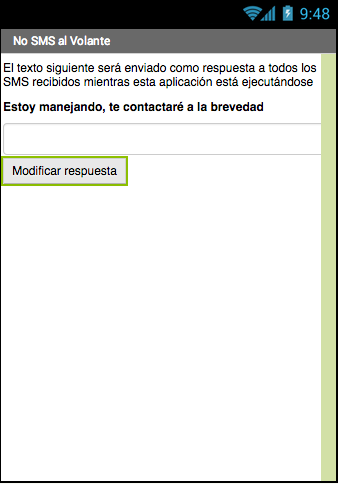
\includegraphics[scale=0.5]{NoSMS1}
\caption{La aplicación \appName{No SMS al Volante}.}
\label{fig:NoSMS1}
\end{figure}


\subsection*{Qué Aprenderás}

Es una aplicación más compleja que las de las actividades previas.
Entonces, la vas a construir paso por paso, una funcionalidad a la
vez, empezando con el mensaje de respuesta automática. Aprenderás
sobre:

\begin{itemize}

\item El componente \component{EnviarTexto} para enviar mensajes de
  textos y procesar los mensajes recibidos.

\item Un formulario de entrada para someter el mensaje de respuesta
  personalizada.

\item El componente de base de datos \component{TinyDB} para guardar o
  preservar el mensaje personalizado después del cierre de la
  aplicación.

\item El evento \block{Screen.Inicializar} para cargar la respuesta
  personalizada cuando la aplicación se comienza a ejecutar.

\item El componente \component{TextoAVoz} para escuchar el texto de
  los mensajes recibidos en voz alta.

% \item El componente \component{SensorDeUbicación} para repartir su
%   ubicación actual.
\end{itemize}

% \subsection*{Para Comenzar}

% Para que funcione esta aplicación, necesitas tener en tu teléfono un
% módulo para transformar el texto a voz, de nombre \emph{Texto-To-Speech-Extended} alta, el }{Text-To-Speech
% Extended}{. }

% {This module is included in Android version 2 or higher, but if you are
% running an Android 1.}{x}{~operating system, you'll need to download it
% from the Android Market. On your phone: ~~~~~~~~}

% \begin{enumerate}
% \itemsep1pt\parskip0pt\parsep0pt
% \item
%   {Open the Market app.}
% \item
%   {Search for TTS.}
% \item
%   {Select the app }{Text-To-Speech Extended}{~to
%   install.}\textsuperscript{\hyperref[cmnt59]{{[}bg{]}}}
% \end{enumerate}

% {}

% {Abre el módulo }{Text-To-Speech }{para testear sus funcionalidades.
% Cuando lo abres, selecciona el idioma español. Después, selecciona
% ``Listen to Preview.''}

% {Si no escuchas nada, asegurate que el volumen de tu teléfono es lo
% suficiente alto.También puedes cambiar la voz cambiando el ajuste por la
% propiedad TTS Default Engine.}

% {}

% {Después de haber ajustado el módulo Text-To-Speech, conéctate al sitio
% web App Inventor y empiezas un nuevo proyecto. Llamalo
% ``NoSMSalVolante'' (los nombres de proyectos no pueden tener espacios) y
% pon ``NoSMSalVolante'' como titulo de pantalla. Luego, abre el Blocks
% Editor y conectate al teléfono a través de la red WiFi.}

% {}

\subsection*{Diseñar los componentes}

La interfaz de usuario para esta aplicación es bastante simple: tiene
una etiqueta que muestra la respuesta automática, con una caja de
texto y un botón para agregar un cambio.

También tendrás que seleccionar un componente \component{EnviarTexto},
un componente \component{TinyDB}, y un componente
\component{TextoAVoz}, y un componente
\component{SensorDeUbicación}.Todos aparecerán en la zona de
componentes no visibles. Los componentes de tu proyecto debieran verse
como en la~\Cref{fig:NoSMS2}.

\begin{figure}[H]
\vspace{3em}
\centering
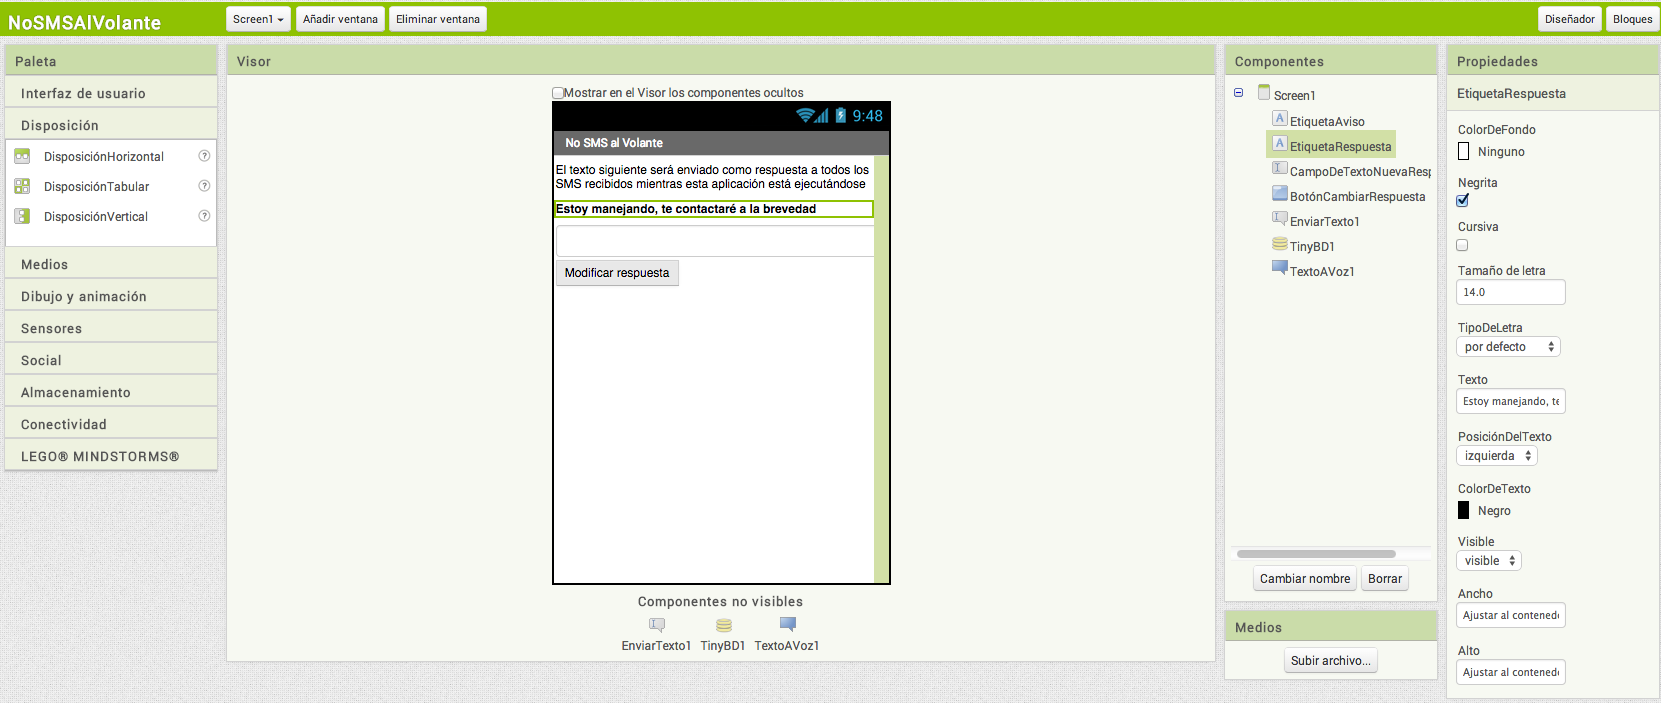
\includegraphics[scale=0.3]{NoSMS2}
\caption{La aplicación \appName{No SMS al Volante} en el
  \componentDesigner.}
\label{fig:NoSMS2}
\end{figure}

Puedes construir la interfaz de usuario mostrada en
la~\Cref{fig:NoSMS2} seleccionando los componentes listados en
la Tabla~\ref{tab:NoSMS1}.

\begin{table}
\centering
\begin{footnotesize}
\begin{tabular}{|l|l|m{4cm}|}

\hline

Tipo Componente & Nombre & Propósito\\

\hline

Etiqueta & EtiquetaAviso & Dice al usuario cómo
funciona la aplicación\\

\hline

Etiqueta & EtiquetaRespuesta & La respuesta que
se enviará al remitente del mensaje de texto recibido\\

\hline

CampoDeTexto & CampoDeTextoNuevaRespuesta & El usuario ingresará una
respuesta personalizada aquí\\

\hline

Botón & BotónCambiarRespuesta & El usuario presiona el botón para
cambiar la respuesta\\

\hline

EnviarTexto & EnviarTexto1 & Procesa los mensajes de texto\\

\hline

TinyDB & TinyDB1 & Almacena la respuesta en una base de datos\\

\hline

TextoAVoz & TextoAVoz1 & Lee en voz alta los mensajes recibidos\\

\hline

% SensorDeUbicación & SensorDeUbicación1 & Siente dónde está el
% dispositivo\\
% \hline
  \end{tabular}
\end{footnotesize}
\caption{Todos los componentes de la aplicación \appName{No SMS al Volante}.}
\label{tab:NoSMS1}
\end{table}
%
Luego debes configurar los componentes de la siguiente manera:

\begin{itemize}

\item \property{Texto} de \component{EtiquetaAviso}: ``El texto
  siguiente será enviado como respuesta a todos los SMS recibidos
  mientras esta aplicación está ejecutándose''.

\item \property{Texto} de \component{EtiquetaRespuesta}: ``Estoy
  manejando, te contactaré a la brevedad''. Selecciona la propiedad
  \property{Negrita}.

\item \property{Texto} de \component{CampoDeTextoNuevaRespuesta}:
  (Deja el campo de texto en blanco para que el usuario pueda escribir
  en él).

\item La \property{Pista} de \component{CampoDeTextoNuevaRespuesta}:
  ``Escribir texto de nueva respuesta''.

\item \property{Texto} de \component{BotónCambiarRespuesta}:
  ``Modificar respuesta''.

\end{itemize}

\subsection*{Agregar Comportamiento a los Componentes}

Empezarás por programar el comportamiento de la respuesta automática
con texto básico, y luego añadiras funcionalidades de manera sucesiva.

\subsubsection*{Programar una respuesta automática}

Para el comportamiento de la respuesta automática, utilizarás el
componente \component{EnviarTexto} de \AppInventor. Puedes imaginar
que este componente es una pequeña persona dentro de tu teléfono que
sabe leer y escribir texto. Para leer textos, el componente usa el
block de evento \block{EnviarTexto.MensajeRecibido}. Puedes
seleccionar este bloque y color otros bloques adentro para ver lo que
pasaría cuando un mensaje de texto es recibido. En el caso de la
aplicación que vamos a programar, queremos enviar de manera automática
una respuesta de texto escrito anteriormente.

Para programa el texto de la respuesta, colocaras un bloque
\block{EnviarTexto1.EnviarMensaje} dentro del controlador de eventos
\block{EnviarTexto1.MensajeRecibido}. El bloque
\block{EnviarTexto.EnviarMensaje} envía el texto, pero debes con
anterioridad especificar qué texto hay que enviar y a quién hay que
enviarlo, antes de utilizar este bloque. La Tabla~\ref{tab:NoSMS2}
muestra todos los bloques que necesitarás para programar el
comportamiento de respuesta automática, y la~\Cref{fig:NoSMS3} muestra
cómo deben conectarse en el \blockEditor.

\begin{table}
\centering
\begin{footnotesize}
\begin{tabular}{|l|m{7cm}|}
\hline
Bloque & Propósito\\ \hline
\block{EnviarTexto1.MensajeRecibido} & El controlador de evento que se
  gatilla cuando el teléfono recibe un mensaje de texto.\\\hline

\block{poner EnviarTexto1.NúmeroDeTeléfono} & Configurar el número de
teléfono al cual se enviará el mensaje.\\\hline

\block{tomar número} & El número de teléfono de la persona que
envió el mensaje recibido.\\\hline

\block{poner EnviarTexto1.Mensaje} & Configurar el mensaje que será
enviado.\\\hline

\block{EtiquetaRespuesta.Texto} & El mensaje que el usuario configuró
para ser enviado.\\\hline

\block{EnviarTexto1.EnviarMensaje} & Enviar el mensaje.\\\hline
  \end{tabular}
\end{footnotesize}
\caption{Bloques para enviar una respuesta automática.}
\label{tab:NoSMS2}
\end{table}

\begin{figure}[H]
\centering
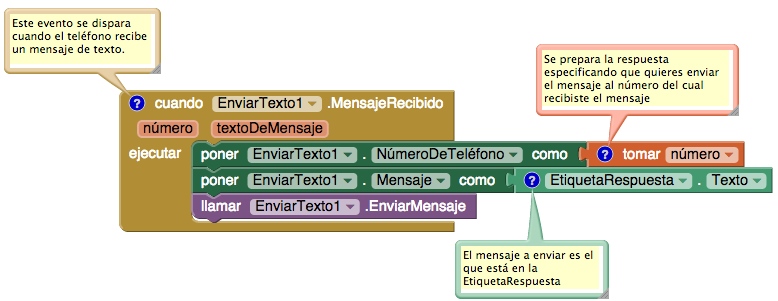
\includegraphics[scale=0.5]{NoSMS3}
\caption{Contestar a un mensaje de texto entrante}
\label{fig:NoSMS3}
\end{figure}

Cuando el teléfono recibe un mensaje de texto, el evento
\block{EnviarTexto1.MensajeRecibido} se activa. Como lo muestra
la~\Cref{fig:NoSMS3}, el número de teléfono del que llama (el
remitente) se encuentra en el argumento \parameter{número}, y el
mensaje de texto recibido está en el
argumento \parameter{textoDeMensaje}.

Para la respuesta automática, la aplicación necesita mandar un mensaje
de texto al remitente. Para enviar el texto, tienes que configurar dos
propiedades del componente \component{EnviarTexto1}: el número de
teléfono del destinatario, \property{EnviarTexto1.NúmeroDeTeléfono}, y
el mensaje a enviar, \property{EnviarTexto1.Mensaje}.

Para hacer esto, asigna el valor del número de teléfono del remitente
en \property{NúmeroDeTeléfono} y el texto que escribiste en
\component{EtiquetaRespuesta} (``Estoy manejando, te contactaré a la
brevedad'') en \component{EnviarTexto1.Mensaje}. Una vez que estas
propiedades están configuradas, la aplicación llama a
\component{EnviarTexto1.EnviarMensaje} para enviar la respuesta.

Los comentarios constituyen una parte sumamente importante en la
programación. Otros programadores pueden usarlos para informarse sobre
el código. Puedes añadir comentarios con un click derecho sobre un
bloque y seleccionando ``Añadir Comentario''. Una vez que has añadido
comentarios, puedes mostrarlos o esconderlos haciendo un click en el
signo de interrogación azul que aparece. No es obligatorio que
incluyas comentarios en tu aplicación, los incluimos en el ejemplo
para ayudar a describir cada bloque y lo que hace.

La mayoría de las personas utilizan comentarios para documentar cómo
están construyendo su aplicación; los comentarios explican cómo el
programa funciona, pero no modifican la aplicación ni la hacen
comportarse de manera distinta. Los comentarios son importantes, tanto
para ti (estás construyendo tu aplicación y seguramente la modificaras
en el futuro), como para otras personas que podrían querer
personalizarla. Todo el mundo está de acuerdo para decir que un
software cambia y se transforma a menudo. Por esta razón, comentar el
código es muy importantes en ingeniería de software, y especialmente
con software libre (de código abierto o \emph{open source}) como
\AppInventor.

\paragraph{Prueba tu Aplicación!} Necesitarás un segundo teléfono para
probar la aplicación. Pídele a tus compañeros que te manden un mensaje
de texto mientras tienes la aplicación ejecutándose. El teléfono de tu
compañero debe recibir la respuesta automática.

\subsubsection*{Escribir una respuesta personalizada}

En esta segunda etapa, vamos a añadir bloques para que el usuario
pueda escribir su propia respuesta personalizada. En el
\componentDesigner añadiste un componente
\component{CampoDeTextoNuevaRespuesta} que es donde el usuario podrá
entrar su respuesta personalizada. Cuando el usuario presiona el botón
\component{BotónCambiarRespuesta} tienes que copiar el texto ingresado
en \component{CampoDeTextoNuevaRespuesta} hacia la etiqueta
\component{EtiquetaRespuesta}, cuyo texto se usa para contestar
automáticamente los mensajes de texto.

La Tabla~\ref{tab:NoSMS3} muestra los bloques que necesitarás para
transferir una nueva respuesta personalizada hacia la
\component{EtiquetaRespuesta}.

\begin{table}
\centering
\begin{footnotesize}
\begin{tabular}{|l|m{7cm}|}
\hline
Bloque & Propósito\\ \hline
\block{BotónCambiarRespuesta.Click} & El usuario presiona el botón
para configurar la nueva respuesta.\\\hline

\block{poner EtiquetaRespuesta.Texto} & Cambia el texto de la etiqueta
por la nueva respuesta.\\\hline

\block{CampoDeTextoNuevaRespuesta} & El usuario ingresa aquí el texto
de la nueva respuesta.\\\hline
  \end{tabular}
\end{footnotesize}
\caption{Bloques para respuesta personalizada.}
\label{tab:NoSMS3}
\end{table}

Piensa en el funcionamiento de un formulario típico: primero entras un
texto en un campo de texto, luego presionas un botón para decir al
sistema que procese el texto. El formulario de esta aplicación no es
distinto para nada!

La~\Cref{fig:NoSMS4} muestra cómo utilizar los bloques para procesar
la respuesta al evento \block{BotónCambiarRespuesta.Click} cuando el
usuario presiona dicho botón.

\begin{figure}[H]
\centering
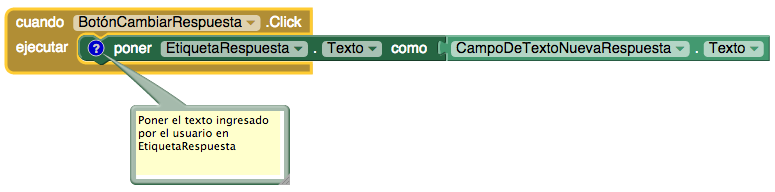
\includegraphics[scale=0.5]{NoSMS4}
\caption{Cambiar la respuesta cuando el usuario entra un
mensaje personalizado.}
\label{fig:NoSMS4}
\end{figure}

En este caso, el controlador de evento copia lo que el usuario
escribió en \component{CampoDeTextoNuevaRespuesta} hacia la
\component{EtiquetaRespuesta}. Recuerda que la
\component{EtiquetaRespuesta} corresponde al mensaje que va a ser
enviado en la respuesta automática, entonces quieres estas seguro que
este mensaje es el nuevo mensaje personalizado que el usuario acaba de
entrar.

\paragraph{Prueba tu Aplicación!} Ingresa una respuesta personalizada
y valídala. Luego pide a un compañero que te envíe un mensaje de texto
mientras ejecutas la aplicación. ¿Recibió tu compañero la respuesta
correcta?

\subsubsection*{Almacenar la Respuesta Personalizada en una Base de Datos}

{Ya tienes una excelente aplicación, pero con un defecto: si el
  usuario entra una respuesta personalizada, cierra la aplicación y
  después la ejecuta de nuevo, la nueva respuesta automática no
  aparecerá. Este no es el comportamiento que el usuario esperaría;
  quieren ver la respuesta personalizada cuando lanzan la aplicación
  de nuevo. Para que esto pase, tienes que almacenar
  \emph{persistentemente} la respuesta personalizada.

  Podrías pensar que poner datos en la propiedad
  \component{EtiquetaRespuesta.Texto} corresponde técnicamente a
  almacenarlos, pero el problema es que estos datos almacenados en
  propiedades de componentes son datos \emph{transitorios}.  Los datos
  transitorios son como tu memoria a corto plazo; el teléfono los
  olvida apenas cierra la aplicación. Si quieres que la aplicación
  recuerde algo de manera persistente, tienes que transferir los datos
  desde la memoria a corto plazo (una propiedad de componente o una
  variable) a la memoria a largo plazo (una base de datos).

  Para almacenar datos de manera persistente, usarás el componente
  \component{TinyDB} que guarda datos en una base de datos que se
  encuentra en el dispositivo Android. \component{TinyDB } provee dos
  funciones: \block{GuardarValor} y \block{ObtenerValor}. La primera
  permite a la aplicación almacenar información en la base de datos
  del dispositivo, mientras la segunda permite a la aplicación acceder
  a datos que están ya almacenados.

  Para varias aplicaciones, usarás el esquema siguiente:

\begin{enumerate}

\item Almacenar datos en la base de datos cada vez que el usuario
  entra un valor nuevo.

\item Cuando la aplicación se inicia, cargar las datos desde la base
  de datos y guardarlos en variables o propiedades.
\end{enumerate}

Empezarás por modificar el controlador de evento
\component{BotónCambiarRespuesta.Click} para que almacene datos de
manera persistente, usando los bloques listados en la
Tabla~\ref{tab:NoSMS4}.

\begin{table}
\centering
\begin{footnotesize}
\begin{tabular}{|l|m{7cm}|}
\hline
Bloque & Propósito\\ \hline
\block{TinyDB1.GuardarValor} & Almacena la respuesta personalizada en
la base de datos del teléfono.\\\hline

Bloque de texto \block{``mensajeRespuesta''} & Nombre o etiqueta para
identificar el mensaje de respuesta en la base de datos.\\\hline

\block{EtiquetaRespuesta.Texto} & Aquí se muestra el mensaje de
respuesta.\\\hline

  \end{tabular}
\end{footnotesize}
\caption{Bloques para almacenar la respuesta personalizada
  con TinyDB.}
\label{tab:NoSMS4}
\end{table}

Esta aplicación utiliza \component{TinyDB} para tomar el texto que está en
\component{EtiquetaRespuesta} y almacenarlo en la base de datos. Como
lo muestra la~\Cref{fig:NoSMS5}, cuando almacenas datos en la base de
datos, tienes que marcar o etiquetar tus datos, para poder
recuperarlos posteriormente. En este caso la etiqueta es
``mensajeRespuesta''.

\begin{figure}[H]
\centering
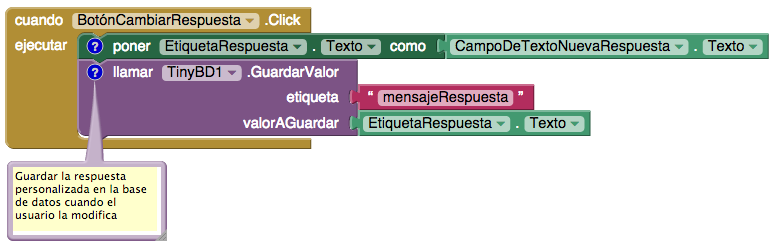
\includegraphics[scale=0.5]{NoSMS5}
\caption{Almacenando la respuesta personalizada de manera
  persistente.}
\label{fig:NoSMS5}
\end{figure}

\subsubsection*{Recuperar la Respuesta Personalizada al Abrir la Aplicación}

La razón por la cual queremos almacenar la respuesta personalizada en
la base de datos es para poder recuperar la respuesta de vuelta la próxima
vez que el usuario abre la aplicación. Como ya hemos mencionado
anteriormente, \AppInventor provee un bloque de evento que se activa
cuando la aplicación se abre: \component{
evento especial que está activado cuando la aplicación se abre:
}{Screen1.Inicializar}. Si seleccionas este bloque y colocas otros
bloques adentro, éstos serán ejecutados justo al abrir la aplicación.

Para esta aplicación, el controlador de evento \component{Screen1.Inicializar
} debe averiguar si una respuesta personalizada está almacenada en
la base de datos. De ser así, la respuesta personalizada debería ser
cargada usando la función \component{TinyDB.ObtenerValor}. Los bloques
principales que necesitarás se muestran en la Tabla~\ref{tab:NoSMS5}.

\begin{table}
\centering
\begin{footnotesize}
\begin{tabular}{|l|m{7cm}|}
\hline
Bloque & Propósito\\ \hline
Definir variable global \variable{respuesta} &
Una variable temporal para almacenar los datos obtenidos.\\\hline

Bloque de texto vacío &
El valor inicial para la variable, puede ser cualquier cosa.\\\hline

\block{TinyDB1.ObtenerValor} &
Obtiene el valor almacenado en la base de datos.\\\hline

Bloque de texto \block{``mensajeRespuesta''} &
Argumento para el parámetro \parameter{etiqueta} de la función
\component{TinyDB1.ObtenerValor}. Asegúrate que la etiqueta es la
misma que la usada para guardar los datos anteriormente.\\\hline

Bloque \block{longitud} (sección ``Texto'') &
Para chequear si el texto obtenido de la base de datos tiene largo
mayor que 0 (o sea, si está vacío o no).\\\hline

  \end{tabular}
\end{footnotesize}
\caption{Bloques para cargar los datos de vuelta al abrir la aplicación}
\label{tab:NoSMS5}
\end{table}

La~\Cref{fig:NoSMS6} muestra el código necesario. Para entenderlo,
tienes que visualizar a un usuario abriendo la aplicación por primera
vez, ingresando una respuesta personalizada, y abriendo la aplicación
varias veces después. La primera vez que el usuario abre la
aplicación, no habrá ninguna respuesta personalizada en la base de
datos a cargar, entonces tienes que poner la respuesta preescrita
(respuesta por defecto) en ~\component{EtiquetaRespuesta}. Al ejecutar
la aplicación las próximas veces, cargarás las respuestas
personalizadas almacenadas desde la base de datos y las colocaras en
\component{EtiquetaRespuesta}.

\begin{figure}[H]
\centering
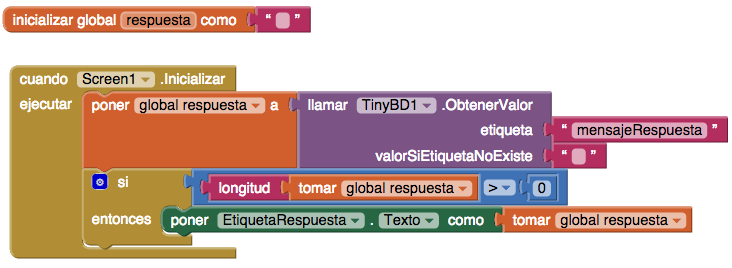
\includegraphics[scale=0.5]{NoSMS6}
\caption{Cargando la respuesta personalizada desde la base de datos en
  la inicialización de la aplicación.}
\label{fig:NoSMS6}
\end{figure}

Cuando la aplicación empieza, el evento \block{Screen1.Inicializar} se
activa. La aplicación llama a \block{TinyDB1.ObtenerValor} con una
etiqueta ``mensajeRespuesta''---la misma etiqueta que utilizaste
cuando almacenaste la respuesta personalizada del usuario un tiempo
atrás. El valor correspondiente se coloca en la variable
\variable{respuesta} para que puedas inspeccionarla antes de poner el
valor en \component{EtiquetaRespuesta}.

\paragraph{Pregunta:} ¿por qué razón quieres poder inspeccionar el
valor obtenido de la base de datos antes de mostrarlo como respuesta
personalizada al usuario?  {}

\paragraph{Respuesta:} \component{TinyDB} retorna un texto vacío si no
hay datos correspondiente a la etiqueta especificada como argumento en
la base de datos. No habrá datos la primera vez que la aplicación se
abre; y seguirá siendo así hasta que el usuario entre una respuesta
personalizada.

La variable \variable{response} contiene el valor almacenado en la
base de datos, entonces podemos usar un bloque condicional para
averiguar si el largo de lo que fue retornado desde la base de datos
es mayor a 0. Si es así, la aplicación sabe que \component{TinyDB}
retornó algo, y el valor correspondiente puede ser colocado en
\component{EtiquetaRespuesta}. Si el largo no es superior a 0, la
aplicación sabe que no hay una respuesta personalizada que haya sido
almacenada, entonces no modifica la \component{EtiquetaRespuesta},
dejando así la respuesta por defecto.

\paragraph{Prueba tu Aplicación!} No puedes testear este
comportamiento en vivo, por que la base de datos de \component{TinyDB}
se borra cada vez haces ``Connect AI Companion'' para recargar la
aplicación.

Lo que debes hacer es seleccionar ``Generar'' y luego ``App (generar
código QR para el archivo .apk)''; después escanea el codigo de barra,
y luego descargas la aplicación en tu teléfono. Una vez que la
aplicación está instalada, ingresa una nueva respuesta
personalizada. Después cierra la aplicación y vuelve a
abrirla. ¿Aparece el mensaje personalizado que pusiste?

\subsubsection*{Leer en Voz Alta el Mensaje de Texto Recibido}

Ahora modificarás la aplicación de tal manera que cuando recibes un
mensaje de texto, se habla en voz alta el número de teléfono del
remitente y su mensaje de texto. La idea es que cuando estás manejando
y escuchas un mensaje de texto llegar, va a estar tentado de leer el
texto incluso si sabes que la aplicación va a mandar una respuesta
automática. Con la funcionalidad de texto-a-voz, puedes escuchar el
texto y seguir manejando.

Los dispositivos Android vienen con capacidades de texto-a-voz y
\AppInventor provee un componente, \component{TextoAVoz}, que hablará
cualquier texto que le des (Nota: por ``texto'' se entiende una
secuencia de letras, cifras y puntuación, no una mensaje de texto
obligatoriamente). El componente \component{TextoAVoz} es muy simple
de usar: solamente llamas su función \block{Hablar} y le das como
argumento el texto que quieres que el teléfono pronuncie. Por ejemplo,
la función mostrada en la~\Cref{fig:NoSMS7} diría ``Hola Mundo''.

\begin{figure}[H]
\centering
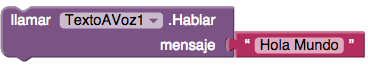
\includegraphics[scale=0.5]{NoSMS7}
\caption{Bloques para decir ``Hola Mundo'' en voz alta.}
\label{fig:NoSMS7}
\end{figure}

Para la aplicación \appName{No SMS al Volante}, necesitarás hacer
hablar un mensaje más complicado, que contiene el texto recibido y el
mensaje de la persona que lo mandó. En vez de conectar un objeto
estático como el bloque de texto ``Hola Mundo'', conectarás un bloque
\block{unir} (de la sección ``Texto''). El bloque \block{unir} te
permite combinar piezas separadas de texto (o números u otros
caracteres) en un solo objeto de texto.

Necesitarás llamar a \block{TextoAVoz.Hablar} dentro del controlador
de eventos \component{EnviarTexto.MensajeRecibido} que programaste
anteriormente. Los bloques que programaste hace algunos pasos atrás
manejan el evento ajustando las propiedades
\property{NúmeroDeTeléfono} y \property{Mensaje}, y luego enviando la
respuesta de texto. Debes extender este controlador de evento
añadiendo los bloques de la Tabla~\ref{tab:NoSMS6}.

\begin{table}
\centering
\begin{footnotesize}
\begin{tabular}{|l|m{7cm}|}
\hline
Bloque & Propósito\\ \hline
\block{TextoAVoz.Hablar} &
Pronuncia en voz alta el mensaje de texto recibido.\\\hline

Bloque \block{unir} &
Construye el texto completo que será leído en voz alta.\\\hline

Bloque de texto \block{``Mensaje recibido de''} &
Las primeras palabras que se dirán.\\\hline

\block{tomar númeroDeTeléfono} &
El número del remitente del mensaje recibido.\\\hline

Bloque de texto \block{``. El mensaje es''} &
Poner un punto después del número de teléfono ,y luego decir ``El
mensaje es''.\\\hline

\block{tomar mensajeDeTexto} & El mensaje recibido.\\\hline

  \end{tabular}
\end{footnotesize}
\caption{Bloques para hablar el texto entrante en voz alta.}
\label{tab:NoSMS6}
\end{table}

Después de enviar la respuesta automática, la aplicación llama a la
función \block{TextoAVoz.Hablar}, como lo muestra
la~\Cref{fig:NoSMS8}. Puedes conectar cualquier objeto de texto en el
parámetro \parameter{mensaje}. En este caso,se usa \block{unir}{join}
para construir las palabras por ser habladas. \emph{Concatena} (o
añade, o pega juntos) el texto ``Mensaje recibido de '' y el número de
teléfono del remitente, seguido por el texto ``. El mensaje es'', y
finalmente el mensaje recibido. Entonces, si el texto ``Hola'' fue
enviado desde el número ``111-2222'', el teléfono diría: ``Mensaje
recibido de 111-2222. El mensaje es Hola''.

\begin{figure}[H]
\centering
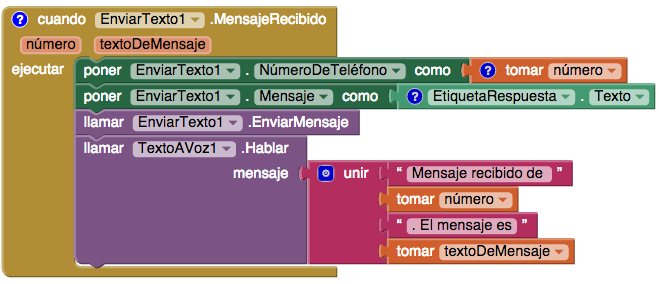
\includegraphics[scale=0.5]{NoSMS8}
\caption{Hablando en voz alta el texto recibido.}
\label{fig:NoSMS8}
\end{figure}

\paragraph{Prueba tu Aplicación!} Necesitarás que alguien te envíe un
mensaje de texto mientras ejecutas la aplicación. ¿Lee en voz alta el
mensaje tu teléfono? ¿Recibe el otro teléfono la respuesta automática
correcta?

\subsection*{Resumen}

En este tutorial has desarrollado los siguientes conceptos:

\begin{itemize}

\item El componente \component{EnviarTexto} puede ser utilizado para
  mandar mensajes de texto y para procesar los mensajes de texto
  recibidos. Antes de llamar a \block{EnviarTexto.EnviarMensaje} debes
  ajustar las propiedades de \property{NúmeroDeTeléfono} y
  \property{Mensaje}. Para contestar a un texto recibido, tienes que
  programar el controlador de eventos
  \component{EnviarTexto.MensajeRecibido}.

\item El componente \component{TinyDB} se utiliza para almacenar
  información de manera persistente---en la base de datos del
  teléfono---para que los datos puedan ser cargados cada vez que la
  aplicación se abre.

\item El componente \component{TextoAVoz} toma cualquier objeto de
  texto y lo habla en voz alta.

\item El bloque \block{unir} se usa para juntar (\emph{concatenar})
  distintos textos separados en un solo objeto de texto.

\end{itemize}


\section{Material de Apoyo}

\subsection*{Listas}

Las listas son un tipo de objeto que permite almacenar varios valores
al mismo tiempo. También la idea de las listas es poder ejecutar
tareas repetitivas sobre cada uno de los elementos de una lista. Por
ejemplo, podemos usar una lista para enviar un mensaje de texto a 3
compañeros.

\subsubsection*{Solución sin Usar Listas}

Consideremos una aplicación con un botón
\component{BotónEnviarMensajes}. La~\Cref{fig:Listas1} muestra cómo
enviar 3 mensajes de texto usando el componente
\component{EnviarTexto}.

\begin{figure}[H]
\vspace{3em}
\centering
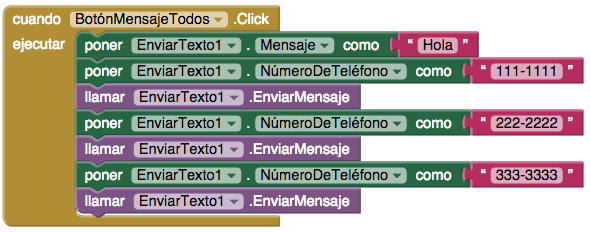
\includegraphics[scale=0.5]{Listas1}
\caption{Enviar mensaje de texto a 3 números de teléfono, sin usar listas.}
\label{fig:Listas1}
\end{figure}

Como puedes ver, la solución simplemente consiste en repetir 3 veces
la configuración y ejecución del bloque
\block{EnviarTexto.EnviarMensaje}. ¿Qué pasa ahora si queremos enviar
el mensaje a 4 amigos? ¿Y si son 10? ¿Y si son 100? Ya no es muy
entretenido agregar tantos bloques, y además hay mucha posibilidad de
error.

\subsubsection*{Solución Usando Listas}

Utilizando listas podemos tener una parte del código que es general,
sin importar la cantidad de destinatarios de nuestro mensaje, y una
parte particular, que es la lista de los números de teléfono. Para
esta solución debes seguir los siguientes pasos:

\begin{itemize}

\item Definir una variable global para guardar los números de
  teléfono.

\item Conectar un bloque \block{construye una lista}, y presionar el
    ícono azul para darle 3 campos.

  \item Conectar 3 bloques de texto a la lista, que serán los 3
    números de teléfono.

  \item Utilizar el bloque \block{por cada elemento en la lista}. Este
    bloque va a \emph{recorrer} o \emph{iterar} por cada uno de los
    elementos de la lista, y para cada uno de ellos ejecutará el
    contenido dentro de su parámetro ``ejecutar''.

    Por lo tanto, si hay 3 elementos en la lista, los bloques dentro
    del \block{por cada ...} serán ejecutados 3 veces. En la ejecución
    de estos bloques, el parámetro \parameter{elemento} hace
    referencia al elemento de la lista que está siendo procesado.
\end{itemize}

El código de la aplicación usando listas se muestra en
la~\Cref{fig:Listas2}.

\begin{figure}[H]
\centering
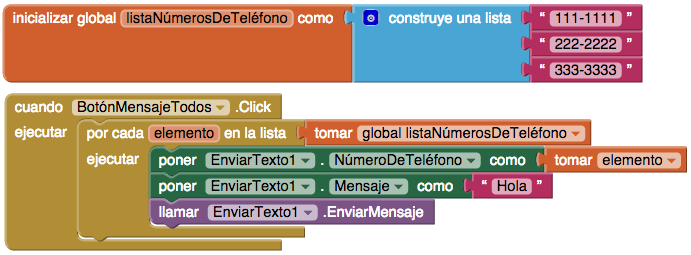
\includegraphics[scale=0.5]{Listas2}
\caption{Enviar mensaje de texto a 3 números de teléfono, usando listas.}
\label{fig:Listas2}
\end{figure}

Las listas de datos se encuentran en muchas aplicaciones! Por ejemplo,
cuando usas Facebook tienes una lista de tus amigos, una lista de tus
mensajes, etc. En tus aplicaciones, podrías querer \emph{monitorear}
los números de teléfono de tus amigos, una lista de tus puntos en un
juego, o el número de kilómetros que corriste cada día de la semana
pasada.

Dado que en casi todos los sistemas de software hay listas de datos
involucradas \AppInventor, como la mayoría de los lenguajes de
programación, provee funcionalidades para procesar los elementos de
una lista y realizar la misma operación en cada elemento. Con
\AppInventor usas un bloque \block{por cada elemento...}. Veamos otro
ejemplo.

\paragraph{Ejemplo: ¿Cómo sumar una lista de números?}

En el ejemplo anterior, la lista de números de teléfono está
fija. Pero en general, las aplicaciones trabajan con listas dinámicas
generadas con datos ingresados por el usuario. Por ejemplo, en una
aplicación deportiva el usuario ingresaría el número de kilómetros que
corre cada día. Consideremos como ejemplo de esto la lista de
la~\Cref{fig:Listas3}, que muestra cómo sumar los kilómetros
recorridos cada día.

\begin{figure}[H]
\vspace{3em}
\centering
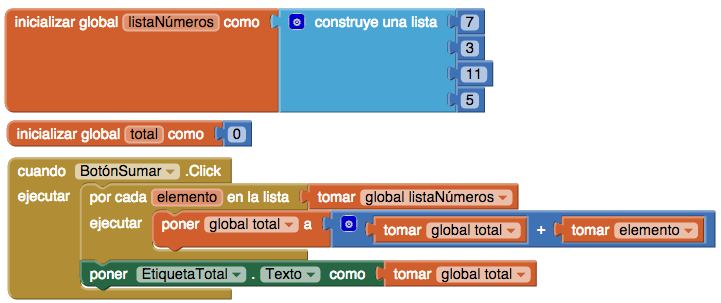
\includegraphics[scale=0.5]{Listas3}
\caption{Aplicación que suma los kilómetros diarios recorridos por el
  usuario.}
\label{fig:Listas3}
\end{figure}

En este ejemplo podemos observar lo siguiente:

\begin{itemize}
\item El bloque \block{por cada} se usa para iterar sobre los números
  de la lista.

\item La variable \variable{total} se usa para calcular el resultado
  total de la suma. Se inicializa con su valor en 0.

\item El parámetro \parameter{elemento} primero tiene valor 7, luego
  3, luego 11, y finalmente 5.

\item En la primera iteración, \variable{total} tiene su valor previo
  (0) más el valor de \parameter{elemento} (7), entonces se ajusta el
  \variable{total} a $0+7 = 7$.

\item En la segunda iteración, \variable{total} tiene su valor previo
  (7) más el valor de \parameter{elemento} (3), entonces se ajusta el
  \variable{total} a $7+3 = 10$.

\item Después de la tercera iteración \variable{total} vale 21, y
  después de la cuarta iteración \variable{total} vale 26, y se
  termina la ejecución del bloque \block{por cada}.

\item Luego de la iteración, se escribe el total en una etiqueta para
  mostrarlo al usuario.

\end{itemize}

\subsection*{Datos Persistentes}

Cuando ingresas información en tu página de Facebook o en otras
aplicacines, tú esperas que esta información este guardada para que la
proxima vez que visites la página, lo que pusiste siga ahí! Lo mismo
pasa con \AppInventor: a medida que trabajas en tus proyectos, puedes
cerrar la página para luego volver y continuar con el trabajo en el
lugar en que te quedaste. Cuando la información se guarda y aparece la
próxima vez que visitas una página o abres una aplicación, se dice que
los datos son \emph{persistentes}. En contraste, los datos que sólo
duran mientras la página o aplicación están abiertos se conoce como
datos \emph{transitorios}. Puedes pensarlo también como la memoria a
largo plazo y la memoria a corto plazo de las aplicaciones.

En \AppInventor, la memoria a corto plazo o transitoria se expresa en
las propiedades de los componentes y en las variables que uses en tus
aplicaciones. Para los datos persistentes debes usar el component
\component{TinyDB}, que provee dos funciones esenciales:

\begin{itemize}

\item \block{TinyDB.GuardarValor} que recibe una \emph{etiqueta} que
  identifica los datos almacenados, y el valor que quieres almacenar
  en la base de datos.

\item \block{ObtenerValor}, que busca en la base de datos si hay
  información asociada a una etiqueta específica. Si hay datos, los
  devuelve, y si no los hay te entrega un valor por defecto que tú
  debes configurar.

\end{itemize}

Cuando creas aplicaciones con datos persistentes debes preocuparte
primero de guardar los datos! Pero además, debes considerar lo
siguiente:

\begin{itemize}

\item ¿Cuándo es necesario recuperar los valores desde la base de
  datos? En general, es buena práctica recuperarlos justo antes de que
  sean necesarios. En el tutorial era necesario cargar los datos
  cuando la aplicación se inicializa, pero no necesariamente debe ser
  siempre así.

\item ¿Qué pasa si no hay datos almacenados? Tu aplicación debe
  considerar el uso de valores por defecto mientras no haya
  información almacenada en la base de datos.

\end{itemize}

\section*{Preguntas y Discusión}

Considera las soluciones siguientes para mandar un mensaje de texto a
una serie de números de teléfono, que se mostraron anteriormente en
la~\Cref{fig:Listas1} y la~\Cref{fig:Listas2}.

\begin{enumerate}

\item Si tienes que añadir un elemento a la lista de números de
  teléfono, ¿para qué solución sería más fácil realizar el cambio?

\item ¿Cuántas funciones (llamadas y ajustes de configuración) se
  ejecutan en la primera solución? Sin contar el bloque \block{por
    cada} y el controlador de evento.

\item ¿Cuántas funciones se ejecutarían si en la lista hubiera $n$ elementos?

\item El código de la primera solución podría ser más eficiente, es
  decir, que podrían ejecutarse menos bloques si cambiaras algunas
  cosas. ¿Qué bloques moverías y por qué?

\item Las aplicaciones anteriores están diseñadas para un usuario en
  específico. Es decir, una sola lista de teléfonos para un usuario
  del teléfono. ¿Si quisieras que la aplicación fuera más general,
  cómo la cambiarías?

\item Si quieres hacer que la lista de números de teléfono sea
  dinámica, es decir que quieres permitir al usuario ingresar y
  cambiar los números de teléfono que van a recibir un mensaje, cuál
  solución sería mejor? ¿Por qué?

\end{enumerate}

\section*{Ejercicios de Personalización}

Te invitamos a realizar los siguientes desafíos de programación!
También puedes personalizar la aplicación a tu gusto!

\begin{enumerate}

\item Escribe una versión de \appName{No SMS al Volante} que deja al
  usuario definir respuestas personalizadas para ciertos números de
  teléfono. Por ejemplo: tu mejor amigo te manda un mensaje de texto,
  contestas con un mensaje, pero para cualquier otra persona contestas
  con otro mensaje. Necesitarás añadir bloques condicionales para
  distinguir los números de teléfono de los remitentes.

\item Escribe una versión de la aplicación que emite una una alarma
  cuando un mensaje de texto es recibido desde un número que se
  encuentra dentro de una lista especial de notificación.

\item Escribe una aplicación que manda mensajes de texto a todos los
  usuarios de una lista, pero permite al usuario entrar y cambiar los
  números de la lista y cambiar el mensaje a enviar. Los datos deben
  ser persistentes.

\item Escribe una aplicación que guarda notas escritas por el
  usuario. Las notas deben poder editarse, y los datos deben ser
  persistentes. ¿Cómo implementarías que las notas puedan ser
  borradas?

\end{enumerate}